%  A simple AAU report template.
%  2015-05-08 v. 1.2.0
%  Copyright 2010-2015 by Jesper Kjær Nielsen <jkn@es.aau.dk>
%
%  This is free software: you can redistribute it and/or modify
%  it under the terms of the GNU General Public License as published by
%  the Free Software Foundation, either version 3 of the License, or
%  (at your option) any later version.
%
%  This is distributed in the hope that it will be useful,
%  but WITHOUT ANY WARRANTY; without even the implied warranty of
%  MERCHANTABILITY or FITNESS FOR A PARTICULAR PURPOSE.  See the
%  GNU General Public License for more details.
%
%  You can find the GNU General Public License at <http://www.gnu.org/licenses/>.
%
%  A simple AAU report template.
%  2015-05-08 v. 1.2.0
%  Copyright 2010-2015 by Jesper Kjær Nielsen <jkn@es.aau.dk>
%
%  This is free software: you can redistribute it and/or modify
%  it under the terms of the GNU General Public License as published by
%  the Free Software Foundation, either version 3 of the License, or
%  (at your option) any later version.
%
%  This is distributed in the hope that it will be useful,
%  but WITHOUT ANY WARRANTY; without even the implied warranty of
%  MERCHANTABILITY or FITNESS FOR A PARTICULAR PURPOSE.  See the
%  GNU General Public License for more details.
%
%  You can find the GNU General Public License at <http://www.gnu.org/licenses/>.
%
\documentclass[11pt,twoside,a4paper,openright]{report}
%%%%%%%%%%%%%%%%%%%%%%%%%%%%%%%%%%%%%%%%%%%%%%%%
% Language, Encoding and Fonts
% http://en.wikibooks.org/wiki/LaTeX/Internationalization
%%%%%%%%%%%%%%%%%%%%%%%%%%%%%%%%%%%%%%%%%%%%%%%%
% Select encoding of your inputs. Depends on
% your operating system and its default input
% encoding. Typically, you should use
%   Linux  : utf8 (most modern Linux distributions)
%            latin1 
%   Windows: ansinew
%            latin1 (works in most cases)
%   Mac    : applemac
% Notice that you can manually change the input
% encoding of your files by selecting "save as"
% an select the desired input encoding. 
\usepackage[utf8]{inputenc}
% Make latex understand and use the typographic
% rules of the language used in the document.
\usepackage[english, spanish]{babel}
% Use the palatino font
\usepackage[sc]{mathpazo}
\linespread{1.05}         % Palatino needs more leading (space between lines)
% Choose the font encoding
\usepackage[T1]{fontenc}
%%%%%%%%%%%%%%%%%%%%%%%%%%%%%%%%%%%%%%%%%%%%%%%%
% Graphics and Tables
% http://en.wikibooks.org/wiki/LaTeX/Importing_Graphics
% http://en.wikibooks.org/wiki/LaTeX/Tables
% http://en.wikibooks.org/wiki/LaTeX/Colors
%%%%%%%%%%%%%%%%%%%%%%%%%%%%%%%%%%%%%%%%%%%%%%%%
% load a colour package
\usepackage{xcolor}
\definecolor{aaublue}{RGB}{33,26,82}% dark blue
% The standard graphics inclusion package
\usepackage{graphicx}
% Set up how figure and table captions are displayed
\usepackage{caption}
\captionsetup{%
  font=footnotesize,% set font size to footnotesize
  labelfont=bf % bold label (e.g., Figure 3.2) font
}
% Make the standard latex tables look so much better
\usepackage{array,booktabs}
% Enable the use of frames around, e.g., theorems
% The framed package is used in the example environment
\usepackage{framed}

%%%%%%%%%%%%%%%%%%%%%%%%%%%%%%%%%%%%%%%%%%%%%%%%
% Mathematics
% http://en.wikibooks.org/wiki/LaTeX/Mathematics
%%%%%%%%%%%%%%%%%%%%%%%%%%%%%%%%%%%%%%%%%%%%%%%%
% Defines new environments such as equation,
% align and split 
\usepackage{amsmath}
% Adds new math symbols
\usepackage{amssymb}
% Use theorems in your document
% The ntheorem package is also used for the example environment
% When using thmmarks, amsmath must be an option as well. Otherwise \eqref doesn't work anymore.
\usepackage[framed,amsmath,thmmarks]{ntheorem}

%%%%%%%%%%%%%%%%%%%%%%%%%%%%%%%%%%%%%%%%%%%%%%%%
% Page Layout
% http://en.wikibooks.org/wiki/LaTeX/Page_Layout
%%%%%%%%%%%%%%%%%%%%%%%%%%%%%%%%%%%%%%%%%%%%%%%%
% Change margins, papersize, etc of the document
\usepackage[
  inner=28mm,% left margin on an odd page
  outer=41mm,% right margin on an odd page
  ]{geometry}
% Modify how \chapter, \section, etc. look
% The titlesec package is very configureable
\usepackage{titlesec}
\titleformat{\chapter}[display]{\normalfont\huge\bfseries}{\chaptertitlename\ \thechapter}{20pt}{\Huge}
\titleformat*{\section}{\normalfont\Large\bfseries}
\titleformat*{\subsection}{\normalfont\large\bfseries}
\titleformat*{\subsubsection}{\normalfont\normalsize\bfseries}
%\titleformat*{\paragraph}{\normalfont\normalsize\bfseries}
%\titleformat*{\subparagraph}{\normalfont\normalsize\bfseries}

% Clear empty pages between chapters
\let\origdoublepage\cleardoublepage
\newcommand{\clearemptydoublepage}{%
  \clearpage
  {\pagestyle{empty}\origdoublepage}%
}
\let\cleardoublepage\clearemptydoublepage

% Change the headers and footers
\usepackage{fancyhdr}
\pagestyle{fancy}
\fancyhf{} %delete everything
\renewcommand{\headrulewidth}{0pt} %remove the horizontal line in the header
\fancyhead[RE]{\small\nouppercase\leftmark} %even page - chapter title
\fancyhead[LO]{\small\nouppercase\rightmark} %uneven page - section title
\fancyhead[LE,RO]{\thepage} %page number on all pages
% Do not stretch the content of a page. Instead,
% insert white space at the bottom of the page
\raggedbottom
% Enable arithmetics with length. Useful when
% typesetting the layout.
\usepackage{calc}

%%%%%%%%%%%%%%%%%%%%%%%%%%%%%%%%%%%%%%%%%%%%%%%%
% Bibliography
% http://en.wikibooks.org/wiki/LaTeX/Bibliography_Management
%%%%%%%%%%%%%%%%%%%%%%%%%%%%%%%%%%%%%%%%%%%%%%%%
%\usepackage[backend=bibtex,
%  bibencoding=utf8
%  ]{biblatex}
%\addbibresource{bib/mybib}

%%%%%%%%%%%%%%%%%%%%%%%%%%%%%%%%%%%%%%%%%%%%%%%%
% Misc
%%%%%%%%%%%%%%%%%%%%%%%%%%%%%%%%%%%%%%%%%%%%%%%%
% Add bibliography and index to the table of
% contents
\usepackage[nottoc]{tocbibind}
% Add the command \pageref{LastPage} which refers to the
% page number of the last page
\usepackage{lastpage}
% Add todo notes in the margin of the document
\usepackage[
%  disable, %turn off todonotes
  colorinlistoftodos, %enable a coloured square in the list of todos
  textwidth=\marginparwidth, %set the width of the todonotes
  textsize=scriptsize, %size of the text in the todonotes
  ]{todonotes}

%%%%%%%%%%%%%%%%%%%%%%%%%%%%%%%%%%%%%%%%%%%%%%%%
% Hyperlinks
% http://en.wikibooks.org/wiki/LaTeX/Hyperlinks
%%%%%%%%%%%%%%%%%%%%%%%%%%%%%%%%%%%%%%%%%%%%%%%%
% Enable hyperlinks and insert info into the pdf
% file. Hypperref should be loaded as one of the 
% last packages
\usepackage{hyperref}
\hypersetup{%
	pdfpagelabels=true,%
	plainpages=false,%
	pdfauthor={Author(s)},%
	pdftitle={Title},%
	pdfsubject={Subject},%
	bookmarksnumbered=true,%
	colorlinks=false,%
	citecolor=black,%
	filecolor=black,%
	linkcolor=black,% you should probably change this to black before printing
	urlcolor=black,%
	pdfstartview=FitH%
}% package inclusion and set up of the document
% see, e.g., http://en.wikibooks.org/wiki/LaTeX/Formatting#Hyphenation
% for more information on word hyphenation
\hyphenation{ex-am-ple hy-phen-a-tion short}
\hyphenation{long la-tex}% 
%  A simple AAU report template.
%  2015-05-08 v. 1.2.0
%  Copyright 2010-2015 by Jesper Kjær Nielsen <jkn@es.aau.dk>
%
%  This is free software: you can redistribute it and/or modify
%  it under the terms of the GNU General Public License as published by
%  the Free Software Foundation, either version 3 of the License, or
%  (at your option) any later version.
%
%  This is distributed in the hope that it will be useful,
%  but WITHOUT ANY WARRANTY; without even the implied warranty of
%  MERCHANTABILITY or FITNESS FOR A PARTICULAR PURPOSE.  See the
%  GNU General Public License for more details.
%
%  You can find the GNU General Public License at <http://www.gnu.org/licenses/>.
%
%
%
% see, e.g., http://en.wikibooks.org/wiki/LaTeX/Customizing_LaTeX#New_commands
% for more information on how to create macros

%%%%%%%%%%%%%%%%%%%%%%%%%%%%%%%%%%%%%%%%%%%%%%%%
% Macros for the titlepage
%%%%%%%%%%%%%%%%%%%%%%%%%%%%%%%%%%%%%%%%%%%%%%%%
%Creates the aau titlepage
\newcommand{\aautitlepage}[3]{%
  {
    %set up various length
    \ifx\titlepageleftcolumnwidth\undefined
      \newlength{\titlepageleftcolumnwidth}
      \newlength{\titlepagerightcolumnwidth}
    \fi
    \setlength{\titlepageleftcolumnwidth}{0.5\textwidth-\tabcolsep}
    \setlength{\titlepagerightcolumnwidth}{\textwidth-2\tabcolsep-\titlepageleftcolumnwidth}
    %create title page
    \thispagestyle{empty}
    \noindent%
    \begin{tabular}{@{}ll@{}}
      \parbox{\titlepageleftcolumnwidth}{
        \iflanguage{danish}{%
          \includegraphics[width=\titlepageleftcolumnwidth]{figures/aau_logo_da}
        }{%
          
\includegraphics[width=\titlepageleftcolumnwidth]{figures/logo}
        }
      } &
      \parbox{\titlepagerightcolumnwidth}{\raggedleft\sf\small
        #2
      }\bigskip\\
       #1 &
      \parbox[t]{\titlepagerightcolumnwidth}{%
      \textbf{Abstract:}\bigskip\par
        \fbox{\parbox{\titlepagerightcolumnwidth-2\fboxsep-2\fboxrule}{%
          #3
        }}
      }\\
    \end{tabular}
    \vfill
    \iflanguage{danish}{%
      \noindent{\footnotesize\emph{Rapportens indhold er frit tilgængeligt, men offentliggørelse (med kildeangivelse) må kun ske efter aftale med forfatterne.}}
    }{%
      \noindent{\footnotesize\emph{}}
    }
    \clearpage
  }
}

%Create english project info
\newcommand{\englishprojectinfo}[8]{%
  \parbox[t]{\titlepageleftcolumnwidth}{
    \textbf{Title:}\\ #1\bigskip\par
    \textbf{Theme:}\\ #2\bigskip\par
    \textbf{Project Period:}\\ #3\bigskip\par
    \textbf{Project Group:}\\ #4\bigskip\par
    \textbf{Participant(s):}\\ #5\bigskip\par
    \textbf{Supervisor(s):}\\ #6\bigskip\par
    \textbf{Copies:} #7\bigskip\par
    \textbf{Page Numbers:} \pageref{LastPage}\bigskip\par
    \textbf{Date of Completion:}\\ #8
  }
}

\newcommand{\spanishprojectinfo}[8]{%
	\parbox[t]{\titlepageleftcolumnwidth}{
		\textbf{Título:}\\ #1\bigskip\par
		\textbf{Periodo del projecto:}\\ #3\bigskip\par
		\textbf{Participantes:}\\ #5\bigskip\par
		\textbf{Supervisores:}\\ #6\bigskip\par
		\textbf{Copias:} #7\bigskip\par
		\textbf{Número de páginas:} \pageref{LastPage}\bigskip\par
		\textbf{Fecha final:}\\ #8
	}
}

%Create danish project info
\newcommand{\danishprojectinfo}[8]{%
  \parbox[t]{\titlepageleftcolumnwidth}{
    \textbf{Titel:}\\ #1\bigskip\par
    \textbf{Tema:}\\ #2\bigskip\par
    \textbf{Projektperiode:}\\ #3\bigskip\par
    \textbf{Projektgruppe:}\\ #4\bigskip\par
    \textbf{Deltager(e):}\\ #5\bigskip\par
    \textbf{Vejleder(e):}\\ #6\bigskip\par
    \textbf{Oplagstal:} #7\bigskip\par
    \textbf{Sidetal:} \pageref{LastPage}\bigskip\par
    \textbf{Afleveringsdato:}\\ #8
  }
}

%%%%%%%%%%%%%%%%%%%%%%%%%%%%%%%%%%%%%%%%%%%%%%%%
% An example environment
%%%%%%%%%%%%%%%%%%%%%%%%%%%%%%%%%%%%%%%%%%%%%%%%
\theoremheaderfont{\normalfont\bfseries}
\theorembodyfont{\normalfont}
\theoremstyle{break}
\def\theoremframecommand{{\color{gray!50}\vrule width 5pt \hspace{5pt}}}
\newshadedtheorem{exa}{Example}[chapter]
\newenvironment{example}[1]{%
		\begin{exa}[#1]
}{%
		\end{exa}
}% my new macros

\usepackage{listings}
\usepackage{color}
\usepackage[utf8]{inputenc}
\usepackage[round, numbers]{natbib}

\definecolor{mygreen}{rgb}{0,0.6,0}

\lstset{ %
	backgroundcolor=\color{white},   % choose the background color; you must add \usepackage{color} or \usepackage{xcolor}; should come as last argument
	basicstyle=\scriptsize,        % the size of the fonts that are used for the code
	breakatwhitespace=false,         % sets if automatic breaks should only happen at whitespace
	breaklines=true,                 % sets automatic line breaking
	commentstyle=\color{mygreen},    
	keywordstyle=\color{blue},       % keyword style
	language=Python,                 % the language of the code
	rulecolor=\color{black},         % if not set, the frame-color may be changed on line-breaks within not-black text (e.g. comments (green here))
	tabsize=4,	                   % sets default tabsize to 2 spaces                
}



\begin{document}
%frontmatter
\pagestyle{empty} %disable headers and footers
\pagenumbering{roman} %use roman page numbering in the frontmatter
%  A simple AAU report template.
%  2015-05-08 v. 1.2.0
%  Copyright 2010-2015 by Jesper Kjær Nielsen <jkn@es.aau.dk>
%
%  This is free software: you can redistribute it and/or modify
%  it under the terms of the GNU General Public License as published by
%  the Free Software Foundation, either version 3 of the License, or
%  (at your option) any later version.
%
%  This is distributed in the hope that it will be useful,
%  but WITHOUT ANY WARRANTY; without even the implied warranty of
%  MERCHANTABILITY or FITNESS FOR A PARTICULAR PURPOSE.  See the
%  GNU General Public License for more details.
%
%  You can find the GNU General Public License at <http://www.gnu.org/licenses/>.
%
\pdfbookmark[0]{Front page}{label:frontpage}%
\begin{titlepage}
  \addtolength{\hoffset}{0.5\evensidemargin-0.5\oddsidemargin} %set equal margins on the frontpage - remove this line if you want default margins
  \noindent%
  \begin{tabular}{@{}p{\textwidth}@{}}
    \toprule[2pt]
    \midrule
    \vspace{0.2cm}
    \begin{center}
    \Huge{\textbf{
      Diseño y construcción de un stage de translación en $x$, $y$ y $z$ automatizado.
    }}
    \end{center}
    \vspace{0.2cm}\\
    \midrule
    \toprule[2pt]
  \end{tabular}
  \vspace{4 cm}
  \begin{center}
    {\large
      Documento final
    }\\
    \vspace{0.2cm}
    {\Large
      Juan Barbosa
    }
  \end{center}
  \vfill
  \begin{center}
  Universidad de los Andes \\
  Departamento de Física
  \end{center}
\end{titlepage}
\clearpage
\thispagestyle{empty}
{\small
	En cada pequeño objeto hay un universo. Para ti, Mau.
\strut\vfill % push the content to the bottom of the page
\noindent Escrito en Python y C. El software de código abierto es un software con código fuente que cualquier persona puede inspeccionar, modificar y mejorar.
}
\clearpage
% !TeX spellcheck = es_ANY
\pdfbookmark[0]{Spanish title page}{label:titlepage_es}
\aautitlepage{%
  \spanishprojectinfo{
    Diseño y construcción de un stage de translación en $x$, $y$ y $z$ automatizado.
  }{%
    Scientific Theme %theme
  }{%
    Segundo periodo 2017
  }{%
    XXX % project group
  }{%
   Juan Barbosa
  }{%
    %list of supervisors
    Manu Forero Shelton, PhD
  }{%
    2 % number of printed copies
  }{%
    Diciembre 3, 2017 % date of completion
  }%
}{%department and address
  \textbf{Universidad de los Andes}\\
  Departamento de Física\\
}{% the abstract
  Con el propósito de funcionar con detectores tales como microscopios ópticos de transmisión, fluorescencia o de reflexión, se construye un stage mecánico automatizado capaz de ser controlado desde el computador, con un área de barrido de 13 cm$^2$, y pasos mínimos de 1.5 $\mu$m en todas las direcciones. La velocidad mínima es de 83 $\mu$m/s, y la máxima de 176 $\mu$m/s en modo continuo. El sistema cuenta además con la posibilidad de ingresar tres puntos en foco, para obtener la ecuación de un plano y de esta forma optimizar el enfoque a lo largo del barrido.
  }

\cleardoublepage
\pdfbookmark[0]{Contenido}{label:contents}
\pagestyle{fancy} %enable headers and footers again
\tableofcontents
%mainmatter
\pagenumbering{arabic} %use arabic page numbering in the mainmatter
\chapter{Introducción}\label{ch:introduccion}
La microscopia óptica representa una fracción muy importante de los desarrollos experimentales en campos de gran importancia en la física desde su invención, y se ha convertido en un instrumento vital para un científico que quiera generar aportes significativos en su campo de estudio. Teniendo en cuenta su importancia, se esperaría que el acceso a microscopios de alta potencia y desempeño estuviera a la mano de cualquiera que estuviera dispuesto a usarlo; sin embargo, existe el problema del costo elevado para el desarrollo de microscopia de alto nivel, y se presenta el reto de desarrollar microscopios de un rendimiento alto que pueda ser accesible a cualquiera en términos económicos. Se han hecho muchos esfuerzos en campos como la biología, la química, la física y la medicina con el fin de lograr el cometido de generar la visualización de alta calidad aplicando técnicas no convencionales \cite{Zhang2016} o haciendo uso de dispositivos de tamaño reducido \cite{Coskun2010, Greenbaum2012}. Es importante remarcar que un microscopio de buena calidad no sólo se compone de una buena etapa de detección óptica, sino que en el caos de la presencia de campos de visión muy grandes se debe contar con un stage mecánico que le permita desplazarse a través de toda el área de interés, y esto se vuelve mucho más crítico cuando la resolución es alta y, por lo tanto, se debe ser muy cuidadoso en la velocidad del movimiento de esta  etapa \cite{Abramowitz2015, Kim2008}.

Con este fin, este proyecto busca generar un stage con capacidad de muestrear la totalidad del volumen de una muestra y con bajo costo de fabricación que pueda, en conjunto con una etapa de detección óptica que se ajuste a las dimensiones del mismo, cumplir la función de un microscopio de alto desempeño para la obtención de resultados ópticos. Esto se logró a partir del desarrollo de una etapa de movimiento mecánico en tres dimensiones, que funciona gracias a la presencia de un motor encargado de desplazar el dispositivo en cada dirección, y una serie de desarrollos de código que controlan el movimiento del stage y permiten generar un plano de enfoque para tener en cuenta lo posibles desniveles de la muestra posicionada bajo la etapa de detección. El documento presenta detalladamente los desarrollos anteriormente descritos, presenta un contexto teórico que permite al lector encontrar las bases del desarrollo, presenta resultados en forma de imágenes y métricas de desempeño del movimiento y finaliza con una discusión acerca de cómo esto podría ser implementado y presenta una serie de conclusiones de todo el trabajo realizado.

\section{Marco teórico}
Dentro de las piezas de mayor importancia de un microscopio óptico se encuentra el stage. En la gran mayoría de los casos estos no son motorizados, restringiendo la reproducibilidad de estudios que requieran estudiar el área total de la muestra. Por otro lado la manipulación de un stage, en caso de no realizarse con el debido cuidado puede dar lugar a la descalibración de partes sensibles del microscopio. La velocidad con la que un ser humano puede manipular el stage puede ser relativamente alta, sin embargo está lejos de ser constante, razón por la cual cuando se quieren hacer estudios de larga exposición o que requieran el movimiento constante de la muestra es necesario un stage automatizado.
\begin{figure}[h]
	\centering
	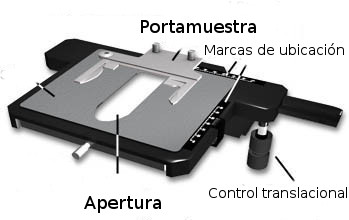
\includegraphics[width=0.5\linewidth]{figures/stage1.jpg}
	\caption{Stage mecánico convencional. Modificado de \cite{Abramowitz2015}.}
\end{figure}

Si bien la automatización permite resolver varios problemas, también se debe tener en cuenta la susceptibilidad a otros. En el caso de un stage en $x$ y $y$ automatizado, al barrer gran cantidad de área se vuelve necesario una preparación de la muestra exhaustiva para limitar cambios significativos en el grosor de la misma que afecten el enfoque sobre el microscopio. Por esta razón se plantea la construcción del stage con una motorización adicional en la dirección $z$.

Existen tres tipos de motores de fácil acceso en el mercado local. Cada uno de ellos con ventajas y desventajas respecto a los demás.
\begin{itemize}
	\item \textbf{Motores de escobillas:} Son los más comunes en el mercado, pues se usan con frecuencia en juguetes, electrodomésticos y accesorios para computadores. Entre sus ventajas se encuentra la velocidad de rotación de los mismos y el torque que generan. Son operados con voltajes análogos. Su desventaja consiste en el control preciso de la posición.  
	\item \textbf{Servo motores:} Los servomotores son usados en aplicaciones donde no se requieren rotaciones completas, pero sí precisión en la ubicación del mismo. Para su manipulación es necesario el uso de frecuencia modulada, es decir realizar pulsaciones sobre salidas digitales. Su gran desventaja es la incapacidad de realizar rotaciones mayores a 180 $^\circ$ y el poco torque que ejercen.
	\item \textbf{Motores de paso:} Este tipo de motores no presenta escobillas, usando un imán y una serie de bobinas separadas entre sí, es posible determinar la orientación del mismo, logrando que este se quede en esa posición hasta que la bobina vecina sea activada. Son ideales para aplicaciones que requieran control de la posición con torques moderados, sin embargo su velocidad de rotación está restringida a la frecuencia de pulsación de cada bobina.
	
	\begin{figure}[h]
		\centering
		\begin{tabular}{ccc}
			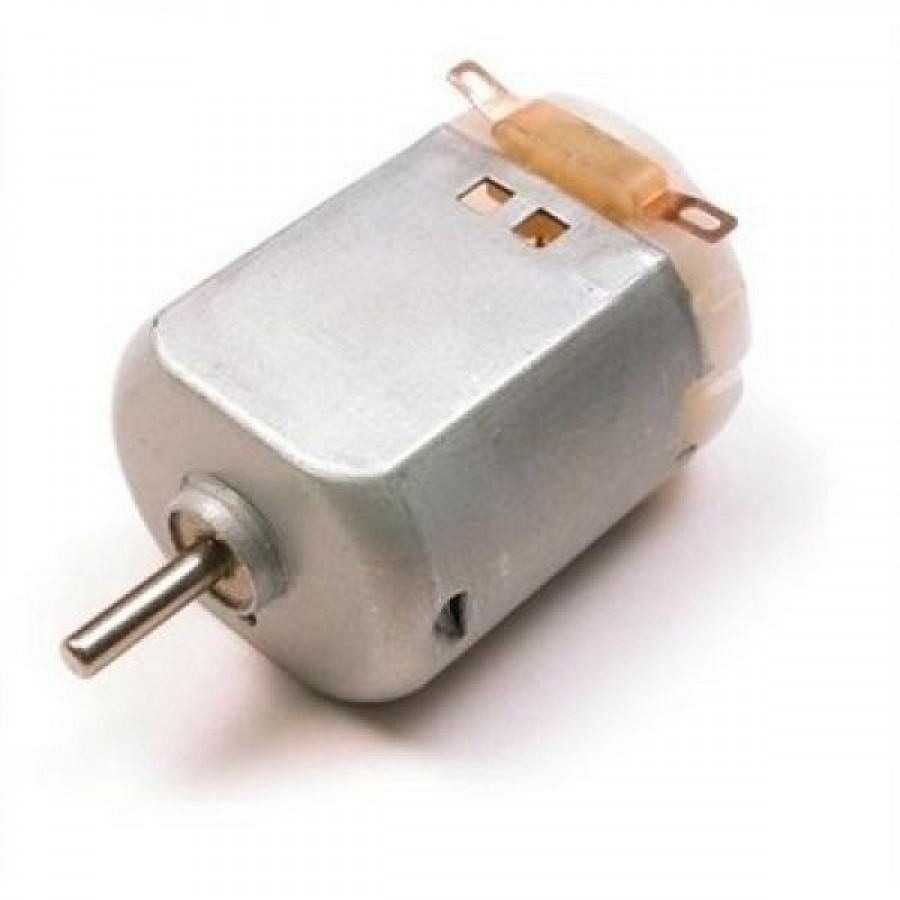
\includegraphics[width = 0.3\linewidth]{figures/brushed.jpg} &
			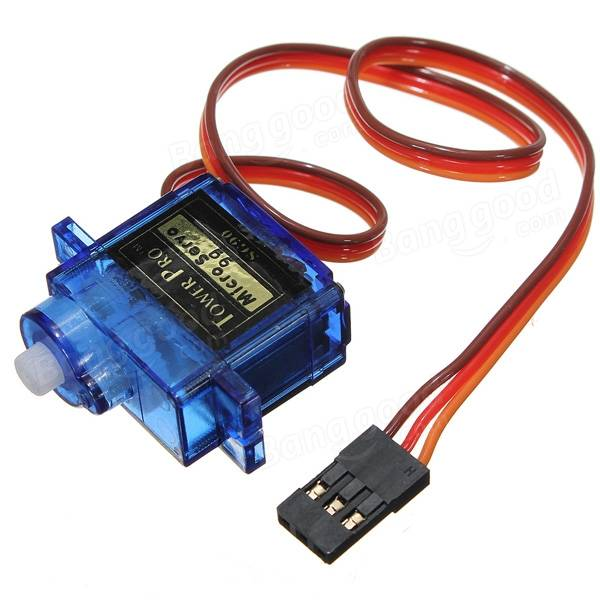
\includegraphics[width = 0.3\linewidth]{figures/stepper.JPG} & 
			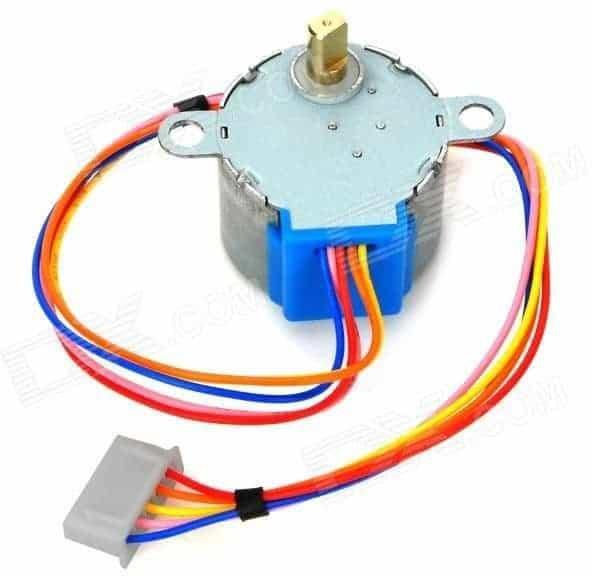
\includegraphics[width = 0.3\linewidth]{figures/paso.jpg}
		\end{tabular}
		\caption{Motores adquiridos para la realización del proyecto. De izquierda a derecha: motor de escobillas, servo y de paso.}
	\end{figure}
\end{itemize}

Finalmente y con el objetivo de realizar el control de los distintos motores, se debe usar un microcontrolador, el cual permita establecer comunicación con el computador para la recepción de instrucciones, y la habilidad de generar los pulsos necesarios para la activación de determinado motor. Entre los requerimientos que este debe tener se encuentran los puertos UART, los cuales permitirán llevar a cabo la comunicación por puerto serial con el computador.
% !TeX spellcheck = es_ANY
\chapter{Fabricación y Resultados}\label{ch:resultados}
\section{Primer modelo}
Tres modelos distintos fueron propuestos para la fabricación del stage. El primero hace uso del sistema de lectura propio de los discos compactos, tales como el CD, DVD y Blu-Ray. Este sistema cuenta con movimiento en dos direcciones, propios de coordenadas cilíndricas. El movimiento en $\theta$ relacionado con traslación en el plano y en $z$ para realizar el enfoque sobre la muestra. 

Usando dos sistemas como el descrito anteriormente y condicionando el experimento a ángulos pequeños es posible obtener un stage aproximado con movimiento $x$, $y$ y $z$.
\begin{equation}
	\begin{matrix}
		x = r\cos\theta \approx r\left(1 - \dfrac{1}{2}\theta^2\right) \\
		y = r\sin\theta \approx r\theta
	\end{matrix}
	\qquad
	\text{donde $r \approx 90$ mm}
\end{equation}

\begin{figure}[h]
	\centering
	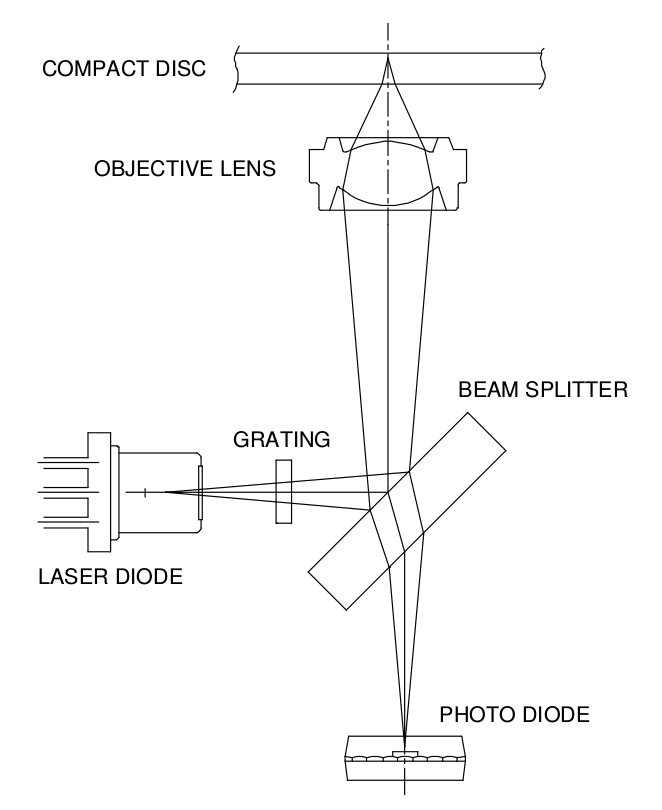
\includegraphics[width=0.3\linewidth]{figures/cdsystem.png}
	\caption{Sistema de detección implementado por la primera versión del stage, el cual hace uso del sistema de lectura de un CD.}
	\label{fig:cdsystem}
\end{figure}

Según el fabricante la distancia máxima de movimiento sobre el plano es de $\pm 0.5$ mm, dando en total $1.0$ mm para translación. En el eje $z$ la distancia máxima es de $\pm$ 0.7 mm, para un total de $1.4$ mm, sin embargo la sensibilidad es de sólo el 20 \%. Usando este stage y aprovechando el interior de los sistemas de lectura de DVDs, se realizó esquema de detección por reflexión, análogo a un microscopio confocal salvo que no existen pinholes el cual se muestra en la \autoref{fig:cdsystem}.

\begin{figure}[h]
	\centering
	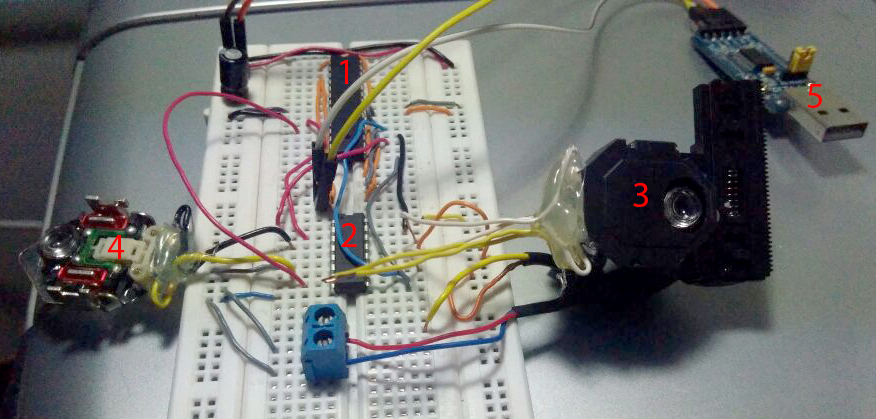
\includegraphics[width=0.8\linewidth]{figures/breadboard}
	\caption{Circuito implementado para el primer stage con etapa de detección. (1) Microcontrolador (Atmega328). (2) Puente H, etapa de potencia para los motores. (3) Sistema \'optico principal con laser y movimiento en $x$. (4) Sistema \'optico con movimiento en $y$. (5) Comunicaci\'on UART.}
	\label{fig:firstsystem}
\end{figure}

El sistema se muestra en la \autoref{fig:firstsystem}. Posicionando el elemento 3 sobre el 4 usando como ayuda una prensa, a la altura donde más pequeño se observó el punto del láser fue posible obtener la imagen que se muestra en la \autoref{fig:firstresults}.

\begin{figure}[h]
	\centering
	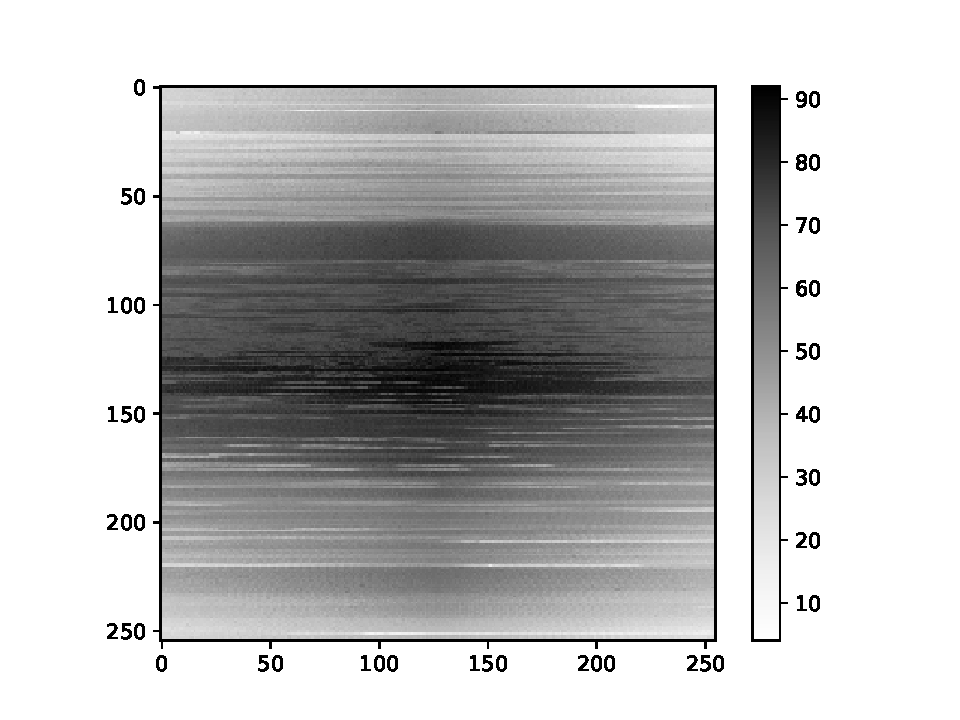
\includegraphics[width=0.62\linewidth]{figures/complete.pdf}
	\caption{Resultados obtenidos usando el primer stage. Se observa la primera línea horizontal de la letra E impresa sobre papel.}
	\label{fig:firstresults}
\end{figure}

El papel con la letra fue tomado de una factura, y se dispuso en la parte superior del lente que se observa en 4, sin ningún tipo de adhesión. De la imagen es importante resaltar que el sistema de detección implementado no cuenta con algún tipo de amplificación, ni de resta del fondo, por lo cual no es posible usar la totalidad de los 10 bits disponibles para la conversión de la señal análoga a digital, y se obtiene únicamente un rango de 0 a 90 valores distintos, lo cual corresponde a 7 bits. Además las condiciones de iluminación del cuarto pudieron alterar los resultados de la medición. En este sentido de implementar un nuevo sistema en el futuro es necesario considerar un sistema de resta en la señal y posterior amplificación de la misma.

Posteriormente y con el objetivo de brindar apoyo en otro proyecto además de simplificar el posicionamiento de la muestra, fueron propuestos dos modelos alternativos.

\section{Segundo modelo}
El segundo modelo propuesto carece de movimiento en la dirección $z$, sin embargo permite un aislamiento del ruido de los motores dado que los mismos se encuentran alejados de la muestra. El movimiento es entonces obtenido al conectar el sistema con los motores usando correas de transporte, los motores serían de paso, conectados al motoreductor que se encuentra a la derecha en la \autoref{fig:secondsystem}, con el objetivo de reducir el tamaño del paso de cada uno de ellos.
\begin{figure}[h]
	\centering
	\begin{tabular}{cc}
		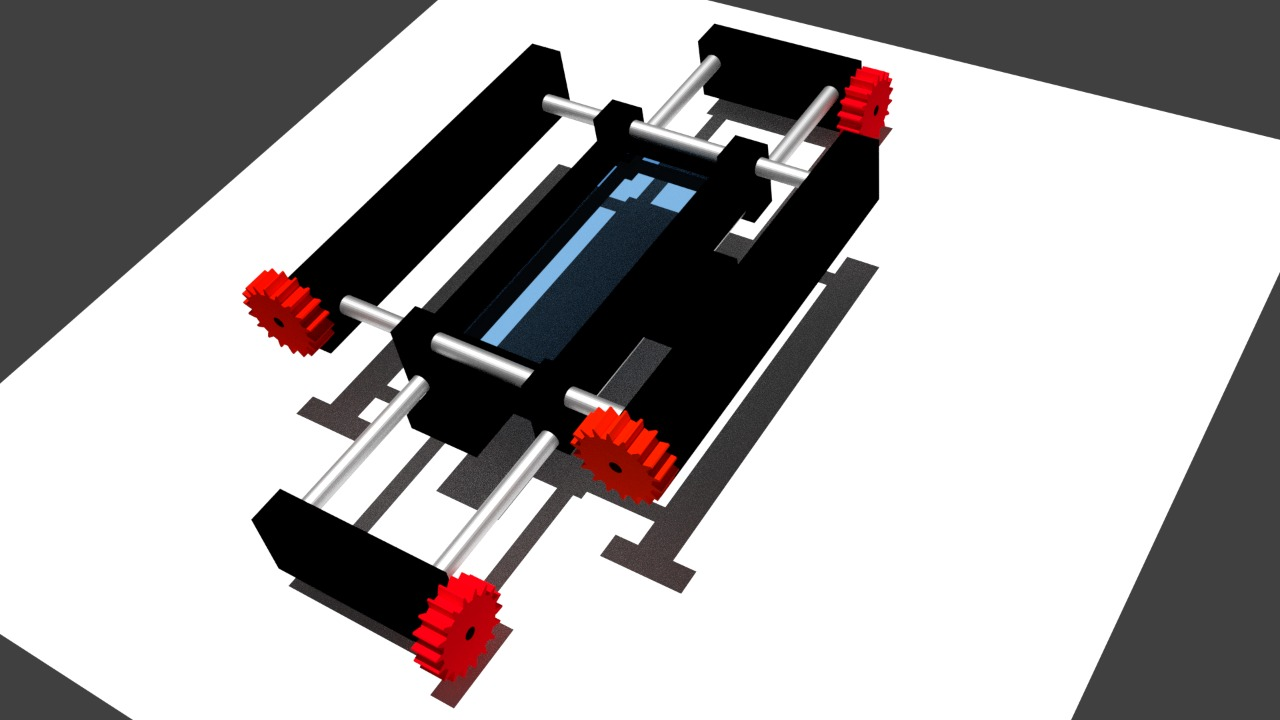
\includegraphics[width=0.45\linewidth]{figures/system2.jpg} & 
		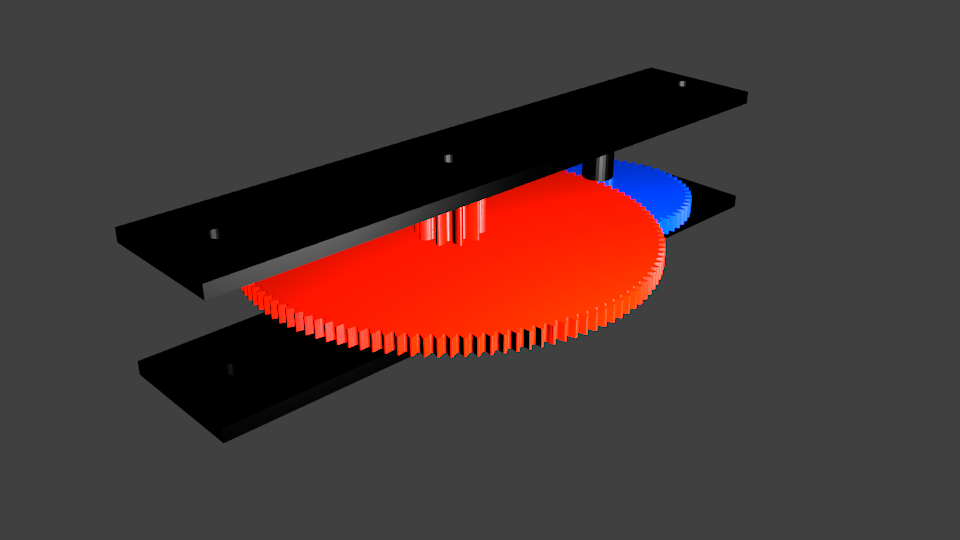
\includegraphics[width=0.45\linewidth]{figures/model2.png}
	\end{tabular}
	
	\caption{Segundo stage propuesto.}
	\label{fig:secondsystem}
\end{figure}

El segundo modelo no fue construido en físico dada la dificultad que se encontró para fabricar las piezas del motoreductor, y su diseño fue reemplazado por el último modelo.

\newpage
\section{Tercer modelo}
Este último fue construido a partir de los planos del Manipulador de BackyardBrains, el cual es de acceso libre, con la posibilidad de realizar modificaciones por los usuarios. Para esto fue necesario la construcción de las piezas del eje $y$ y $z$, dado que las tuercas que se adquirieron eran de dimensiones mucho mayores. Además las bases de los motores fueron diseñadas con el objetivo de obtener un manipulador motorizado. Las piezas fueron diseñadas en Blender, software de uso libre.
\begin{figure}[h]
	\centering
	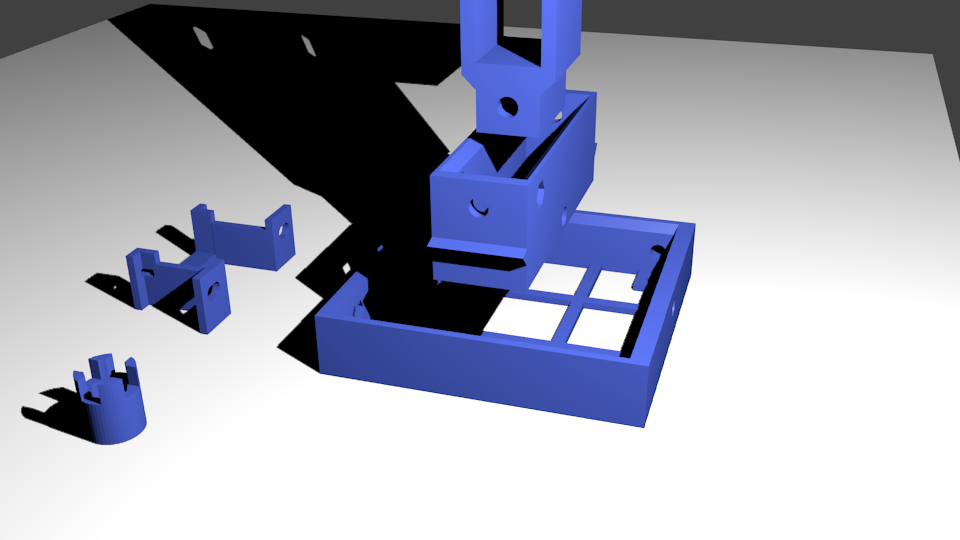
\includegraphics[width=0.9\linewidth]{figures/model3.png}	
	\caption{Tercer stage propuesto.}
	\label{fig:thirdsystem}
\end{figure}

Además de las piezas de impresión, también fue necesario adquirir:
\begin{itemize}
	\item 12 Tornillos M3 de 10 mm.
	\item 2 Tornillos 15/32" de 100 mm.
	\item 1 Tornillo 15/32" de 50 mm.
	\item 12 Tuercas M3.
	\item 6 Tuercas 15/32".
\end{itemize}

Una vez montado el sistema puede moverse las siguientes distancias sobre cada eje, las cuales fueron medidas usando un calibrador Vernier:
\newpage
\begin{table}[h]
	\centering
	\caption{Capacidad en cada dirección del stage.}
	\begin{tabular}{cc}
		\hline
		\textbf{Eje} & \textbf{Distancia (cm)} \\
		\hline
		$x$ & $3.42 \pm 0.01$ \\
		$y$ & $3.90 \pm 0.01$ \\
		$z$ & $1.31 \pm 0.01$ \\
		\hline		
	\end{tabular}
\end{table}

La electrónica es simple, y únicamente fueron necesarios 3 arreglos de transistores Darlington ULN2003, un adaptador de 12 V, y tres motores de paso 28BYJ. El microcontrolador es el mismo usado en el primer modelo, el cual tiene las siguientes tareas: 
\begin{enumerate}
	\item Comunicación con el computador del usuario.
	\item Control de los motores.
\end{enumerate}

El protocolo de comunicación UART establecido envía un mensaje en cada lado de la transmisión de 8 bits, a 4800 baudios. A cada instrucción que envía el computador, el microcontrolador responde \texttt{0xFF} (255 en hexadecimal). Usando el sistema hexadecimal, se usan como primer dígito letras para determinar la identidad del canal, como se muestra en la \autoref{tb:tableUART1}.
\begin{table}[h]
	\centering
	\caption{Identificación de los canales en el protocolo UART.}
	\label{tb:tableUART1}
	\begin{tabular}{cc}
		\hline
		\textbf{Valor} & \textbf{Descripción}\\
		\hline
		A & Canal X \\
		B & Canal Y \\
		C & Canal Z \\
		\hline
	\end{tabular}
\end{table}

Para cada eje es necesario conocer la dirección en la que se desea hacer rotar al motor, la cual es obtenida con el segundo dígito del número hexadecimal.
\begin{table}[h]
	\centering
	\caption{Asignación de la tarea por UART.}
	\label{tb:tableUART2}
	\scriptsize
	\begin{tabular}{cc}
		\hline
		\textbf{Valor} & \textbf{Descripción}\\
		\hline
		0 & Derecha \\
		1 & Izquierda \\
		2 & Pasos: 1 \\
		3 & Pasos: 64 \\
		4 & Pasos: 128 \\
		5 & Pasos: 192 \\
		6 & Pasos: 256 \\
		7 & Pasos: 320 \\
		8 & Pasos: 384 \\
		9 & Pasos: 448 \\
		A & Pasos: 512 \\
		\hline
	\end{tabular}
\end{table}
\newpage

Adicionalmente es posible decirle al microcontrolador que realice varias pasos al motor sin requerir comunicación adicional, es importante decir que el número de pasos para que el motor complete una vuelta es de 512. Con el objetivo de obtener resultados sobre el sistema se realizan mediciones del tiempo requerido para ir y volver hasta el máximo de cada dirección del stage, para varios valores de la resolución (inversos del número de pasos).

En todos los casos se observaron variaciones inferiores al 0.2 \% para resoluciones menores a 9, para el caso de la máxima resolución las variaciones son menores a 1.3 \% en todas las dimensiones, siguiendo la misma forma en todos los casos. Para cada medición se realizaron triplicados, los cuales mostraron desviaciones menores al 0.01\%.

\begin{figure}[h]
	\centering
	\begin{tabular}{cc}
		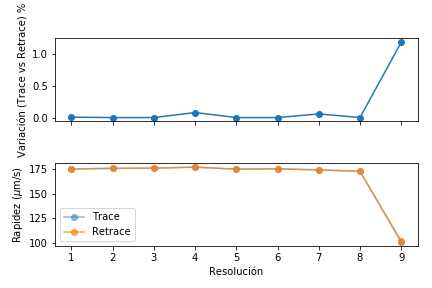
\includegraphics[width=0.5\linewidth]{figures/x.png} & 
		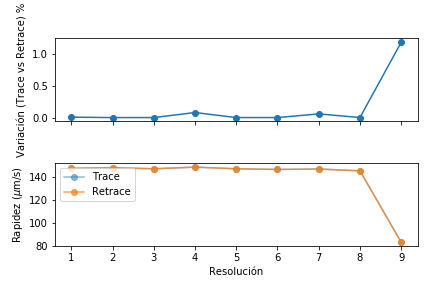
\includegraphics[width=0.5\linewidth]{figures/y.png}
	\end{tabular}
	\caption{Variación y rapidez en función de la resolución para el eje $x$ y $y$, correspondientemente.}
\end{figure}
\begin{figure}[h]
	\centering
	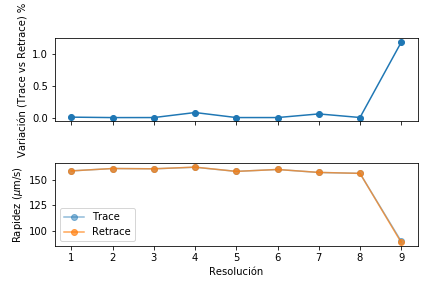
\includegraphics[width=0.45\linewidth]{figures/z.png}
	\caption{Variación y rapidez en función de la resolución para el eje $z$.}
\end{figure}

\newpage
Finalmente y con el objetivo de optimizar el enfoque de un detector sobre una muestra se incluyó en la librería la posibilidad de ingresar 3 puntos $(x, y, z)$ en donde se cumple que la muestra está enfocada, de esta forma es posible obtener un plano que optimiza el enfoque a lo largo de un barrido. Para cada punto del barrido el sistema calcula si debe o no modificarse la altura, por lo que el plano termina en una función de escalones como los que se observan en la \autopageref{fig:plane}, en donde cada cuadro representa las posiciones de medición, el circulo rojo muestra la posición actual del stage.
\begin{figure}[h]
	\centering
	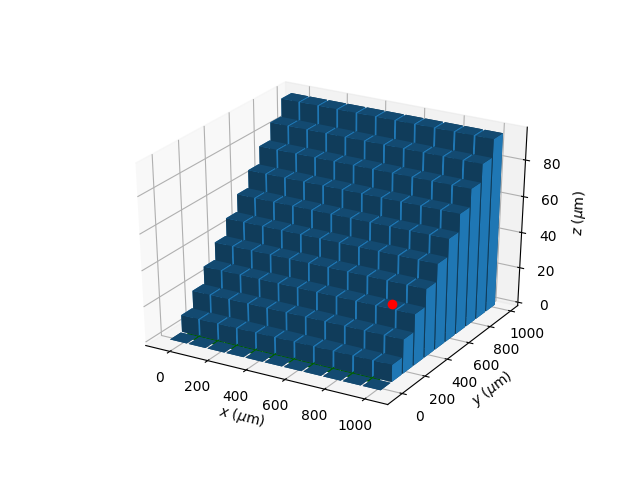
\includegraphics[width=\linewidth]{figures/plane.png}
	\caption{Variación y rapidez en función de la resolución para el eje $z$.}
	\label{fig:plane}
\end{figure}

% !TeX spellcheck = es_ANY
\chapter{Conclusión}\label{ch:conclusion}
Como conclusión de todo el proceso desarrollado se puede entonces asegurar que se construyó un stage de microscopia capaz de hacer barridos en tres dimensiones de una muestra determinada de manera constante y teniendo en cuenta consideraciones de resolución según la etapa de detección a usar. Adicionalmente, el código mediante el cual se pone ene ejecución el proceso considera la toma de tres puntos distribuidos en el área de interés para calcular una ecuación del plano, y por lo tanto tener en cuenta cualquier clase de desnivel en el plano de muestra. Como importante característica se puede remarcar que el stage funciona de tal manera que las medidas se pueden tomar con una velocidad que permita que se tome punto por punto de manera cuidadosa o que se haga un recorrido continuo en las tres dimensiones para abarcar una muestra de tamaño superior en una sola ejecución. Se espera a futuro poder generar una mayor cantidad de pruebas que permitan validar su funcionamiento, mejorar la velocidad de barrido probando una denominación de motor diferente, y como aporte más importante se espera hacer un acople exitoso de la parte mecánica con una etapa de detección con el fin de obtener resultados ópticos y tener un microscopio de bajo costo funcionando en su totalidad. Adicionalmente el proyecto cuenta con una librería para Python, la cual es de acceso libre y puede ser modificada por cualquiera interesado en la misma. 
  \begin{center}
    Juan Barbosa \\
    \href{mailto: js.barbosa10@uniandes.edu.co}{js.barbosa10@uniandes.edu.co}\\
    \href{https://github.com/jsbarbosa}{https://github.com/jsbarbosa}\\
    Universidad de los Andes\\
	Bogotá, Colombia
  \end{center}

\bibliography{bib/mybib}
\bibliographystyle{plainnat}

\appendix
\chapter{Código}\label{ch:userside}
El código fuente del projecto, tanto para el uso del usuario para la obtención de datos, como para la manipulación del microcontrolador al interior del mismo, se encuentra de manera libre en GitHub \footnote{\url{https://github.com/jsbarbosa/miniscope}}. El código es libre, cualquier persona lo puede inspeccionar, modificar y mejorar.

\section{Librería Python (mauscope)}
Disponible en PyPI \footnote{\url{https://pypi.python.org/pypi/mauscope}}(Python Package Index), la instalación se puede llevar a cabo usando el mánager de paquetes de Python (pip) de la siguiente forma:
\begin{lstlisting}
	pip install mauscope
\end{lstlisting}

También es posible descargar la versión de desarrollo desde GitHub seguido de su instalación:
\begin{lstlisting}
	python setup.py install
\end{lstlisting}

\subsection{constants.py}
	\lstinputlisting{../mauscope/constants.py}
\subsection{core.py}
	\lstinputlisting{../mauscope/core.py}
\subsection{commandLine.py}
	\lstinputlisting{../mauscope/commandLine.py}
\subsection{plane.py}
	\lstinputlisting{../mauscope/plane.py}


\section{Ejemplos}

\section{Internal C}\label{ch:internal}
\subsection{motor.c}
\lstinputlisting[language=C]{../microcontroller/motor.c}
\end{document}